% AUTEUR :: Guillaume Van Dessel || SOURCE :: Slides || DATE :: 17.10.2015

\chapter{Champs électromagnétiques} 

 
\section{Introduction}

La première partie du cours de Physique 3 traite des champs électromagnétiques. \\
Comme son nom le suggère, le champ électromagnétique est un \textit{\textbf{champ vectoriel}} spatial
tri-dimensionnel (en toute généralité) dépendant également du \textit{temps}.  Il est la résultante d'une composante \textit{champ 
électrique} et d'une composante \textit{champ magnétique}. 

\section{Lois générales : formulation \textit{intégrale}}

Afin de se figurer comment une telle combinaison de champs se propage dans l'espace et le temps, il est nécessaire d'aborder les grandes 
lois de l'électricité et du magnétisme. 

\subsection{Rappels qualitatifs}
%\begin{fullwidth}



{\huge 1} : Des charges électriques \textit{\textbf{immobiles}} créent un \textit{\textbf{champ électrostatique}}. \\
\textit{Propriété} : Ce champ est \textit{conservatif} et dérive d'un \textbf{potentiel scalaire} \\ 
\textit{Propriété} : \textbf{Force} sur charges électriques en mouvement et stationnaires 

\vspace{5mm}% \hline \vspace{5mm}

{\huge 2} : Des courants constants\sidenote{Déplacements de charges électriques à débit constant}  créent un \textit{\textbf{champ magnétique}} \sidenote{Champ magnétique \textit{d'excitation} $\vec{H}$ qui, couplé à la perméabilité magnétique de l'endroit où il vit donne le champ magnétique d'induction $\vec{B}$} constant. \\
\textit{Propriété} : Des charges en mouvement (accéléré ou non) créent des champs électriques se \textit{déplaçant} \\
\textit{Propriété} : \textbf{Force} sur charges électriques en mouvement uniquement \\

%\vspace{5mm} \hline \vspace{5mm}

\subsection{Théorème de Gauss dans la matière}

Le théorème de Gauss énonce que le flux du \textit{\textbf{champ de déplacement électrique}} \\($\vec{D} = \epsilon_{r}\epsilon_{0}\vec{E} = \epsilon \vec{E}$)
à travers une surface \textit{fermée} vaut exactement la charge électrique comprise dans le volume qu'elle décrit dans l'espace. Cela se traduit par l'équation 

\begin{equation}
 \oint_{S} \vec{D} \cdot d\vec{s} = \int_{V} \rho dv = q_{incl}
 \label{GaussIntegral}
\end{equation}

\subsection{Absence de monopole magnétique}

Cette loi traduit le fait que le champ magnétique (\textit{induit} ou d'\textit{excitation}) n'admet pas de pôle. 
Autrement dit, chaque ligne de champ forme une \textit{courbe} fermée dans l'espace, de telle sorte que le flux 
du champ magnétique à travers une surface \textit{fermée} soit \textbf{nul}.

\begin{equation}
 \oint_{S} \vec{B} \cdot d\vec{s} = 0
 \label{MonoPoleIntegral}
\end{equation}

\subsection{Loi de Lenz-Faraday}

Comme le champ électrostatique dérive d'un potentiel scalaire, par définition mathématique, son intégrale le long 
d'une courbe \textit{fermée} dans l'espace est \textbf{nulle}. % /i\ COMMENT : L'intégrale dépend uniquement du point de départ à d'arrivée, le chemin emprunté n'importe pas. 
\textit{Cependant, si nous avons affaire à un flux magnétique dont la dérivée temporelle est non-nulle, le membre de droite de l'équation n'est plus nul!}

\begin{equation}
 \oint_{C} \vec{E} \cdot d\vec{l} = 0 \hspace{10pt} \mbox{ si } \frac{d\phi}{dt} \not = 0 \Rightarrow  \oint_{C} \vec{E} \cdot d\vec{l} = -\int_{S} \frac{\partial \vec{B}}{\partial t} \cdot d\vec{s}
 \label{PotentielIntegral}
\end{equation}

\subsection{Loi d'Ampère (incomplète)}

La Loi d'Ampère relie l'intégrale de contour du champ magnétique d'excitation au courant traversant la surface décrite par le contour en question. 
Comme nous allons le voir très bientôt, cette Loi, formulée comme ci-dessous (équation 4), est \textbf{incomplète} car elle n'envisage pas tous les cas de figure.
\begin{equation}
 \oint_{C} \vec{H} \cdot d\vec{l} = I + ? = \int_{S} \vec{J} \cdot d\vec{s} + ? 
 \label{AmpèreIntegral}
\end{equation}

\section{Analyse vectorielle}

Nous avons découvert au quadrimestre passé, les concepts de \textit{rotationnel}, \textit{divergence} pour un champ vectoriel et \textit{gradient} pour un champ scalaire.
Nous n'allons pas revenir sur ces concepts fondamentaux mais seulement rappeler deux définitions importantes qui nous permettront de construire les \textbf{lois de Maxwell}. 
Ces dernières sont réellement le ciment de notre connaissance concernant l'électricité et ses phénomènes. \\ 

\subsection{Divergence} 
\begin{marginfigure}[-5cm]
	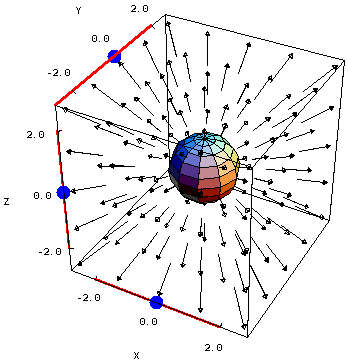
\includegraphics[width=5cm]{rep_div}
	\caption{Représentation de la divergence}
\end{marginfigure}

La divergence d'un champ vectoriel $\vec{F}$ satisfait les équations suivantes : 

\[ \text{div}(\vec{F}) = \nabla \cdot \vec{F} = \lim_{\Delta v \to 0} \frac{\oint_{S} \vec{F} \cdot d\vec{s}}{\Delta v} \]

\[\mbox{Théorème de la divergence : } \hspace{15pt} \oint_{S} \vec{F} \cdot d\vec{s} = \int_{V} (\nabla \cdot \vec{F}) \, dv\]

où $\Delta v$ correspond au volume \textit{infinitésimal} défini par la surface \textit{fermée} $S$.



\subsection{Rotationnel} 
\begin{marginfigure}
	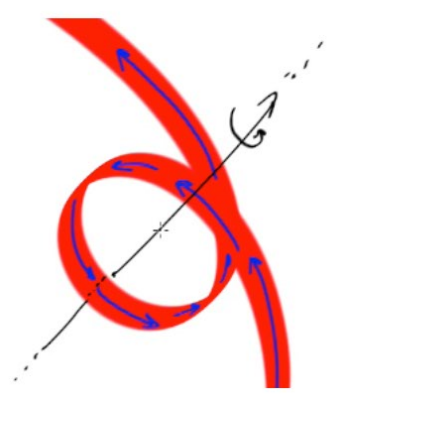
\includegraphics[width=5cm]{rep_rot}
	\caption{Représentation du rotationnel}
\end{marginfigure}

Le rotationnel d'un champ vectoriel $\vec{F}$ satisfait les équations suivantes  

\[  \vec{\text{rot}}(\vec{F}) \cdot \vec{n}   = (\nabla \times \vec{F}) \cdot \vec{n} = \lim_{\Delta s \to 0} \frac{\oint_{C} \vec{F} \cdot d\vec{l} }{\Delta s}\]

\[\mbox{Théorème de Stokes : } \hspace{15pt} \oint_{C} \vec{F} \cdot d\vec{l} = \int_{S} (\nabla \times \vec{F}) \cdot d\vec{s}\]

où $\Delta s$ correspond à la surface (aire) infinitésimale décrite par la courbe fermée $C$. \\
\textbf{NOTE : } le rotationnel est un concept inhérent à un espace tri-dimensionnel, nous pouvons le ramener à un espace de dimension moindre 
mais au delà de 3, il perd son sens.

\subsection{Propriétés des opérateurs différentiels}

Dans ce paragraphe, nous rappelons diverses propriétés des opérateurs différentiels que nous avons étudiées au second quadrimestre. 
\\  

\textit{Le rotationnel d'un champ vectoriel dérivant d'un potentiel scalaire est le champ "nul".} 

\[\nabla \times \nabla V = \vec{0} \] 

\textbf{NOTE : } Le rotationnel du champ électrostatique défini par $\vec{E} = -\nabla V$ est donc par conséquent nul!  \\ 

\textit{La divergence d'un champ vectoriel rotationnel est  "nulle".}  

\[\nabla \cdot (\nabla \times \vec{A})  = 0 \]

\section{Equations de Maxwell}
Désormais, nous avons toutes les informations pour commencer à compléter les équations de Maxwell \sidenote{Enlever les intégrales revient à dire : \textit{\textbf{localement}}, l'équation est valable!}. 
Seule la Loi d'Ampère nécessitera une légère modification à la fin. \\

\begin{center}

\begin{tabular}{|c|c|}

\hline

1 & L'équation (1) devient : $ \oint_{S} \vec{D} \cdot d\vec{s}  =  \int_{V} (\nabla \cdot \vec{D} ) dv =  \int_{V} \rho dv$ \\  
- & $\Rightarrow \forall  \hspace{3pt} \mbox{ vol infinitésimal} \hspace{5pt} (\nabla \cdot \vec{D} ) = \rho$  \\

\hline

2 & L'équation (2) devient : $ \oint_{S} \vec{B} \cdot d\vec{s}  =  \int_{V} (\nabla \cdot \vec{B} ) dv =  \int_{V} 0 dv$ \\ 
- & $\Rightarrow \forall  \hspace{3pt} \mbox{ vol infinitésimal} \hspace{5pt} (\nabla \cdot \vec{B} ) = 0 $ \\

\hline

3 & L'équation (3) devient : $   \oint_{C} \vec{E} \cdot d\vec{l} = \int_{S} (\nabla \times \vec{E}) d\vec{s}= -\int_{S} \frac{\partial \vec{B}}{\partial t} \cdot d\vec{s}$ \\  
- &$ \Rightarrow \forall  \hspace{3pt} \mbox{ surf infinitésimale} \hspace{5pt} (\nabla \times \vec{E} ) = -\frac{\partial \vec{B}}{\partial t}$\\

\hline

\end{tabular}

\end{center}

\subsection{Terme manquant de la loi d'Ampère}

Nous allons ici montrer l'\textit{incohérence} de la loi d'Ampère pour certains cas de figure. \\
Prenons par exemple  le cas d'un circuit RC basique. Nous branchons en série une résistance $\mathcal{R}$ (ne joue pas de rôle particulier mais permet de formaliser les choses) et un condensateur plan $\mathcal{C}$ à une source de tension $\mathcal{V}$. Un courant $I_{c}(t)$ va naitre depuis la source de tension. Il passe à travers la résistance et atteint la borne \textbf{positive}\sidenote{Nous prenons la convention d'un courant de charges positives} du condensateur. Là, les particules sont théoriquement stoppées car le diélectrique présent entre les deux plaques assure une isolation électrique entre ces deux dernières.\sidenote{Jusqu'à une certaine tension de claquage évidemment} Apparait alors une répulsion électrostatique de l'autre côté du condensateur plan  et un même nombre de particules, chargées positivement elles aussi, quitte la borne \textbf{négative} \sidenote{Négative car au fur et à mesure, une polarité négative s'installe étant donné que les particules chargées positivement quittent la paroi}. Si nous appliquons la loi d'Ampère sous forme intégrale en prenant en compte le vecteur densité de courant $\vec{J}$ et une surface définie par un cercle autour du conducteur électrique par lequel transite le courant total $I_{c}(t)$, nous avons alors 

\[  \oint_{C} \vec{H} \cdot d\vec{l} = I_{c}(t) = \int_{S} \vec{J} \cdot d\vec{s} \]

\begin{marginfigure}[0cm]
	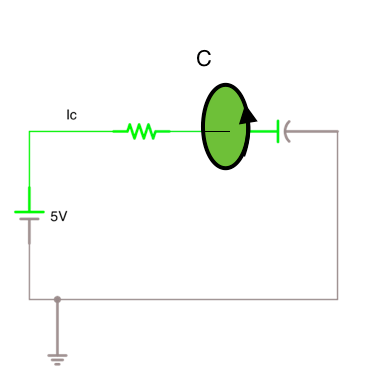
\includegraphics[width=5cm]{circ_ampere_naif}
	\caption{La surface plane définie par C intercepte le courant Ic}
\end{marginfigure}
\begin{marginfigure}[0cm]
	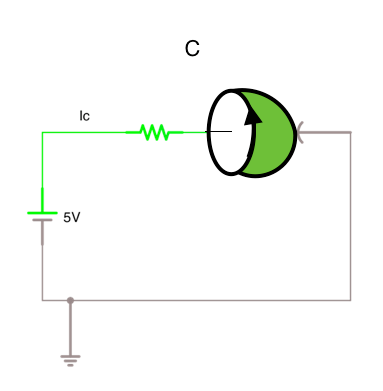
\includegraphics[width=5cm]{circ_ampere_bug}
	\caption{La surface de la semi-sphère définie par C n'intercepte pas le courant Ic}
\end{marginfigure}

Cependant, par la loi d'Ampère, nous pouvons prendre \textit{n'importe quelle surface définie par ce même cercle, le résultat devrait être \textbf{identique}}. \\
Tenons dès lors compte de ce même cercle avec le même circuit mais en changeant la surface considérée pour l'application de l'intégrale de surface de $\vec{J}$. 
Prenons désormais une demi-sphère de cercle principal le cercle autour du conducteur et englobant la borne \textbf{positive} du condensateur. La surface de cette demi-sphère sert
à l'intégration de $\vec{J}$. Nous avons : 

\[  \oint_{C} \vec{H} \cdot d\vec{l} =  \int_{S} \vec{J} \cdot d\vec{s} = I_{out}(t)\] 

où $I_{out}(t)$ représente le courant sortant de la borne \textbf{positive} du condensateur vers l'autre borne. 
Il est évidemment nul, par définition! Dès lors, nous sommes confrontés à une contradiction : $I_{c}(t) = I_{out}(t) = 0?$ 
\\ 

Cette contradiction peut être réglée par le développement suivant tiré des slides :
\[I_{c}(t) = \int_{S} \vec{J} \cdot d\vec{s} = -\frac{dQ_{out}(t)}{dt} = - \int \frac{d \sigma(t)}{dt} ds\] 
où $Q_{out}$ représente la charge de la borne \textbf{négative} du condensateur par où le courant $I_{c}(t)$ est "restitué". \\ 

Comme nous avons pour un condensateur plan les relations suivantes \sidenote{Certaines lettres représentent les normes de vecteurs qui leurs sont associés : Ex : E = || $\vec{E}$ ||} 

\[ E \simeq \frac{V}{d} = \frac{Q}{Cd} = \frac{Qd}{\epsilon S d} = \frac{\sigma}{\epsilon} \Rightarrow \frac{\partial E}{\partial t} = \frac{1}{\epsilon} \frac{\partial \sigma}{\partial t} \]
où $d,V,Q,C,S,\sigma,E$ sont respectivement pour le condensateur la distance entre les deux plaques, la différence de potentiel électrique entre les deux plaques, la charge en valeur absolue de chacune des plaques, 
la capacité, la surface d'une des deux plaques, la densité de charge par plaque et le champ électrique entre les deux plaques. \\ 
Nous pouvons maintenant écrire :

\[ I_{c}(t) = \int_{S} \vec{J} \cdot d\vec{s} = -\int_{SurfOut}( \epsilon \frac{\partial \vec{E}}{\partial t} )\cdot d\vec{s} = \]
\[ = - \int_{SurfOut} (\frac{\partial \vec{D}}{\partial t}) \cdot d\vec{s}  =  \int_{SurfOut} \vec{J}_{D} \cdot d\vec{s}\]
où $SurfOut$ représente la surface de la plaque associée à la borne \textbf{négative} du condensateur.

Entre les deux plaques du condensateur, nous pouvons donc observer une \textit{variation} du champ électrique au cours du temps. Cela implique en réalité une variation de champ magnétique par la même occasion! \\
Posons alors que le terme manquant à notre loi d'Ampère soit $\frac{\partial \vec{D}}{\partial t}$. Ce n'est pas aberrant!
En effet, ce terme est en quelque sorte \textit{relié} à une variation de champ magnétique alors que le champ magnétique apparait dans l'intégrale du terme de gauche de la loi d'Ampère.
Nous aurions donc par la formule de Stokes : 

\[ \oint_{C} \vec{H} \cdot d\vec{l} = \int_{S} (\vec{J} +\frac{\partial \vec{D}}{\partial t}) \cdot d\vec{s} \]
\[ \Rightarrow \forall  \hspace{3pt} \mbox{ surf infinitésimale} \hspace{5pt} (\nabla \times \vec{H} ) = \vec{J} + \frac{\partial \vec{D}}{\partial t}\]

De plus, par la propriété des opérateurs différentiels qui dit que $\text{div}(\vec{\text{rot}}\vec{F}) = 0$, nous pouvons écrire : 

\[ \nabla \cdot (\vec{J} + \frac{\partial \vec{D}}{\partial t}) = 0 \Rightarrow \nabla \cdot \vec{J} = - \nabla \cdot \frac{\partial \vec{D}}{\partial t} = - \frac{\partial \rho}{\partial t}\]

ce qui n'est pas aberrant non plus! Nous avons d'un côté de l'équation, un terme exprimant une \textit{somme de courants sortant en un endroit de l'espace} ($\nabla \cdot \vec{J}$) et de l'autre l'expression de l'\textit{évolution de la densité de charge en cet endroit} ($- \frac{\partial \rho}{\partial t}$). Le signe "-" est tout à fait justifié. Une manière de s'en convaincre est la suivante : si nous avons des courants \textit{positifs}, alors la densité de charge diminuera mais le signe "-" donnera un terme doublement négatif donc \textit{positif}.

\subsection{Expression générale du champ électrique}

Cette sous-section admet un objectif purement théorique. En effet, elle vise à exprimer, sur base de nos constats, le champ électrique de manière formelle. 
Repartons dès lors de la \textit{loi de Lenz-Faraday} écrite sous forme \textit{différentielle}.
Nous pouvons définir un \textit{\textbf{potentiel vecteur}} $\vec{A}$ tel que $\nabla \times \vec{A} = \vec{B}$. \sidenote{Cette affirmation est vraie pour tout champ vectoriel $\vec{B}$ \textit{régulier} et de \textit{divergence nulle} sur un domaine \textit{ouvert et étoilé}.} Dès lors, nous pouvons écrire 

\[\nabla \times \vec{E} = - \frac{\partial \vec{B}}{\partial t} = -\frac{\partial (\nabla \times \vec{A})}{\partial t} = - \nabla \times \frac{\partial \vec{A}}{\partial t} \]
\[\nabla \times (\vec{E} + \frac{\partial \vec{A}}{\partial t}) = \vec{0} \]

Ce qui veut dire, par la propriété différentielle $\vec{\text{rot}}(grad$ $V) = \vec{0}$ que $(\vec{E} + \frac{\partial \vec{A}}{\partial t})$ dérive d'un potentiel scalaire.
Nous supposons alors qu'il s'agit bien du potentiel électrique $\mathcal{V}$. Nous spécifions alors l'équation finale exprimant $\vec{E}$ : 

\[(\vec{E} + \frac{\partial \vec{A}}{\partial t}) = - \nabla \mathcal{V} \Rightarrow \vec{E} = - (\nabla \mathcal{V} + \frac{\partial \vec{A}}{\partial t}) \]
 
 \subsection{Conditions aux interfaces}
 
 Les lois de Maxwell gouvernent aussi la continuité des champs électromagnétiques aux interfaces entre deux milieux aux propriétés électromagnétiques différentes. \\
 
 \begin{marginfigure}[-10cm]\\
 	\normalsize 
 	\label{interface1}
 	\caption{\textit{\textbf{En absence de charges et de courants de surface}} à l'interface: }
	\begin{center}
	
	\begin{tabular}{|ccc|}
		
		\hline
		
		$\vec{D}_{1,n} $ & = & $\vec{D}_{2,n} $ \\ 
		
		$\vec{B}_{1,n} $ & = & $\vec{B}_{2,n} $ \\ 
		
		$\vec{E}_{1,t} $ & = & $\vec{E}_{2,t} $ \\ 
		
		$\vec{H}_{1,t} $ & = & $\vec{H}_{2,t} $ \\ 
		
		\hline
		
	\end{tabular}
	
	%%%%% /!\ PROFESSEURS : Puisque D et E et B et H sont, dans notre théorie, égaux à une constante de proportionnalité près. Pourquoi dans le cas du déplacement électrique et de 
	%%%%% l'induction magnétique impose t'on la continuité de la composante normale à l'interface alors qu'avec le champ électrique et l'excitation magnétique ce sont les composantes tangentielles qui
	%%%%% requièrent la continuité ? Merci d'avance.  
	
	%%%%% /!\ COMMENT : vidéo trouvée expliquant le phénomène : https://www.youtube.com/watch?v=wahmW7h-AKo&feature=youtu.be&t=10m21s
	
	%\includegraphics[height = 130pt, width = 400pt]{milieux.png} 
	
	\end{center}

 \end{marginfigure}
 
 
 Pour démontrer le résultat de la figure \ref{interface1}, partons des équations de Maxwell. On imagine au niveau de l'interface un petit cylindre de section $dS$ (dont l'axe est perpendiculaire à l'interface) et une boucle de longueur $dl$ (dont l'axe est parallèle à l'interface). 
\begin{itemize}
\item Si le champ électrique est purement normal, la loi de Gauss appliquée au cylindre  implique que $\vec{D}_{1}\cdot d\vec{S_1} +  \vec{D}_{2}\cdot d\vec{S_2} = Q_{int} = \rho_S dS$; comme $d\vec{S_1} = \vec{n}dS = -d\vec{S_2}$, on trouve que $\vec{n}\cdot(\vec{D}_{1} - \vec{D}_{2}) = \rho_S$. En l'absence de charges à l'interface, $\rho_S = 0$ et donc, $\vec{n}\cdot(\vec{D}_{1} - \vec{D}_{2}) = 0$, soit ${D}_{1,n} = {D}_{2,n}$.
\item Sur base de la loi sur le flux du magnétique, on trouve de manière similaire pour un champ magnétique purement normal que $\vec{n}\cdot(\vec{B}_{1} - \vec{B}_{2}) = 0$, soit ${B}_{1,n} = {B}_{2,n}$.
\item Si le champ électrique est purement tangentiel, la loi de circulation de $\vec{E}$ sur la boucle donne $\vec{E}_1\cdot d\vec{l_1} + \vec{E}_2\cdot d\vec{l_2} = 0$; comme $d\vec{l_1} = - d\vec{l_2}$, on trouve  ${E}_{1,t} =  {E}_{2,t}$.
\item Si le champ magnétique est purement tangentiel, l'application de la loi d'Ampère sur la boucle donne $\vec{H}_1\cdot d\vec{l_1} + \vec{H}_2\cdot d\vec{l_2} = I_{enc}$. Si un courant de surface $\vec{K}$ existe, alors $I_{enc} = \vec{K} d\cdot{l_1}$, puisqu'un courant de surface est défini en Ampères par mètre de largeur. En l'absence de courant à la surface, on trouve que ${H}_{1,t} =  {H}_{2,t}$.
\end{itemize} 
 
 \begin{marginfigure}[-20cm]
 	\normalsize 
 	\caption{Les conditions aux limites deviennent alors (en toute généralité):}
 	\begin{center}
 		
 		\begin{tabular}{|ccc|}
 			
 			\hline
 			
 			$\vec{n} \cdot (\vec{D}_{1} - \vec{D}_{2}) $ & = & $ \rho_S$ \\ 
 			
 			$\vec{n} \cdot (\vec{B}_{1} - \vec{B}_{2}) $ & = & $ 0 $ \\ 
 			
 			$\vec{n} \times (\vec{E}_{1} - \vec{E}_{2}) $ & = & $ 0$ \\ 
 			
 			$\vec{n} \times (\vec{H}_{1} - \vec{H}_{2}) $ & = & $ \vec{K}$ \\ 
 			
 			\hline
 			
 		\end{tabular}
 	\end{center}
 	
 	En l'absence de charges et courants de surface, $\rho_S = 0$ et $\vec{K} = \vec{0}.$
 	
 	% \textbf{NOTE : } Il y a deux directions $\hat{t}$ car en réalité quand nous %parlons de direction tangentielle à l'interface (Ex : $\vec{H}_{1,t}$), 
 	%nous voulons plutôt signifier: pour la partie tangentielle à l'interface, la %condition de continuité s'applique. Mais comme à la surface de l'interface il %existe un plan entier admettant 
 	%des directions tangentielles, nous devons donc rajouter une deuxième %dimension avec le second vecteur unitaire $\hat{t}$ pointant vers le lecteur.
 \end{marginfigure}

% \includegraphics[height = 150pt, width = 250pt]{interface.png} 
Ces lois sont en fait valables si les champs ne sont pas purement normaux ou tangentiels: il suffit de prendre la projection normale ou tangentielle des champs.\sidenote[][-8cm]{\normalsize \textbf{NOTE : } Il y a une infinité de directions tangentielles à l'interface: dès lors, on ne spécifie pas de vecteur tangentiel comme on le fait pour le vecteur normal, noté $\vec{n}$ et pris par convention comme pointant du milieu 2 vers le milieu 1; quand on parle de direction tangentielle à l'interface (Ex : $\vec{H}_{1,t}$), 
	on veut bien signifier la projection sur l'interface du champ vectoriel: pour la partie tangentielle à l'interface, la condition de continuité s'applique. Une manière élégante de représenter cette projection est d'écrire, par exemple, ${H}_{1,t}\vec{t} = \vec{n} \times \vec{H}_{1}$. } \\ 
% /!\ COMMENT & /!\ PROFESSEURS
  %  Quid de cette phrase ? :) (voir en dessous) 
 %Les champs ne sont donc pas, en toute généralité, continus à une interface ! \\ \\
 

 %\todo{Expliquer illustration divergeance et rotationnel.}
 %\subsection{Résumé (slide)}
 %\includegraphics[height = 300pt, width = 450pt]{CM1.png}